\documentclass{article}

\usepackage{amsmath}
\usepackage{amssymb}
\usepackage{float}
\usepackage{caption}
\usepackage{ngerman}
\usepackage{float}
\usepackage{tabularx}
\usepackage{makecell}
\usepackage{enumitem}
\usepackage{marvosym}
\usepackage{xcolor}
\usepackage{tikz}
%\usetikzlibrary{shapes,arrows,positioning}
\usetikzlibrary{automata,arrows,positioning,calc}
\setlength{\parindent}{0em}
\begin{document}


\section{Lineare Algebra}

\subsection{Definitionen}

Ein \textbf{Kern} (\(Ker(A)\)) existiert, wenn \(\det(A) = 0\).\\
Der Kern einer Matrix A ist die Lösungsmenge von \(A \cdot \vec{v} = \vec{0}\)\\
\(\rightarrow\) LGS=0 durch elem. Zeilenoperationen lösen.\\

Das \textbf{Bild} (\(Im(A)\)) einer Matrix gibt an, welche Menge an Vektoren als Lösungen auftreten können (vgl. Wertebereich bei Funktionen).\\
Das Bild einer Matrix A ist die Lösungsmenge von \(A \cdot \vec{v} = \vec{b}\)\\


Der \textbf{Rang} (\(rank(A)\)) einer Matrix A ist die Anzahl der linear unabhängigen Zeilen- bzw. Spaltenvektoren.\\
Rang = Anzahl der Nichtnullzeilen der Matrix in Zeilenstufenform.\\
\(\rightarrow\) A durch elem. Zeilenoperationen umformen.\\

Die \textbf{Länge} eines Vektors \(\vec{v}\) ist die Wurzel aus dem Skalarprodukt mit sich selbst.\\
\(\rightarrow \|\vec{v}\| = \sqrt{\vec{v} \cdot \vec{v}} = \sqrt{v_1^2 + v_2^2 + \dots + v_n^2}\)\\

Das \textbf{Skalarprodukt} \(\left\langle x, y\right\rangle \) zweier Vektoren ist die Summe der Produkte der jeweiligen Komponenten\\
\(\rightarrow x_1y_1+\cdots + x_dy_d\); man kann damit den von \(x\) und \(y\) eingeschlossenen Winkel als Zahl \(\theta \in [0,\pi]\) berechnen mit: \(\cos \theta = \frac{\left\langle x, y\right\rangle}{\|x\|\cdot \|y\|} \rightarrow\) Zwei Vektoren stehen senkrecht zueinander, wenn \(\left\langle x, y\right\rangle = 0\)\\

\subsection{Determinante}

Spezielle Funktion, die einer \underline{quadratischen} Matrix eine Zahl zuordnet. Diese gibt an, wie sich das Volumen bei der durch die Matrix beschriebenen linearen Abbildung ändert. \\

\begin{itemize}
    \item \(det(A)= 0\rightarrow\) Matrix \(A\) ist nicht invertierbar; ist z.B. der Fall, wenn
    \begin{itemize}
        \item eine Zeile oder Spalte nur aus Nullen besteht
        \item 2 Zeilen/Spalten identisch sind
        \item Zeilen/Spalten ein Vielfaches einer anderen Zeile/Spalte sind.
    \end{itemize}
    \item \(det(I) = 1\)
    \item \(det(A) = det(A^T)\)
    \item \(det\begin{pmatrix}
            \lambda \cdot a & \lambda \cdot b \\
            c & d
        \end{pmatrix} = \lambda \cdot det\begin{pmatrix}
            a & b \\
            c & d
        \end{pmatrix} \rightarrow\) Eine Zeile mit \( \lambda \) multiplizieren
    \item \(det(\lambda\cdot A) = \lambda^n \cdot det(A)\) \(\rightarrow\) Ganze Matrix (\(\mathbb{R}^{nxn}\)) mit \( \lambda \) multiplizieren
    \item \(det(A^{-1}) = det(A)^{-1}=\frac{1}{det(A)}\)
    \item \(det(A\cdot B) = det(A)\cdot det(B)\)
    \item \(det\begin{pmatrix}
            a & b \\
            c & d
        \end{pmatrix} = -det\begin{pmatrix}
            c & d \\
            a & b
        \end{pmatrix}\rightarrow\) Zeilentausch: Vorzeichenwechsel
\end{itemize}



\begin{figure}[H]
    \begin{equation*}
        \det\begin{pmatrix}
        a & b \\
        c & d
        \end{pmatrix}
        = ad - bc
    \end{equation*}
\end{figure}

\begin{figure}[H]
    \begin{equation*}
        \det\begin{pmatrix}
        a & b & c \\
        d & e & f \\
        g & h & i
        \end{pmatrix}
        = aei + bfg + cdh - gec - hfa - ibd
    \end{equation*}
\end{figure}



\subsection{Eigenwerte, Eigenvektoren und Eigenraum}

Eine Zahl \(\lambda\) heißt Eigenwert der Matrix A, wenn es einen Vektor \(\vec{v}\) gibt, der nicht der Nullvektor ist, so dass gilt:

\begin{equation}
    \begin{split}
        A v &= \lambda v \\
        A v - \lambda v &= 0 \\
        (A - \lambda I) v &= 0
    \end{split}
\end{equation}


\subsubsection{Charakteristisches Polynom berechnen}
Anstatt o.g. Gleichungzu lösen: Bestimmung der Nullstellen des charakteristischen Polynoms \(p_A(\lambda)\) der Matrix A.

\begin{equation}
    \begin{split}
    p_A(\lambda) & = \det(A - \lambda E) \\
    & = \begin{vmatrix}
    a_{11} - \lambda & \cdots & a_{1n} \\
    \vdots & \ddots & \vdots \\
    a_{n1} & \cdots & a_{nn} - \lambda
    \end{vmatrix} \overset{!}{=} 0
    \end{split}
\end{equation}

Ergebnis: die Eigenwerte \(\lambda_1, \lambda_2, \dots, \lambda_n\) von A.

\subsubsection{Eigenvektoren berechnen}
Der zu einem Eigenwert \(\lambda_i\) gehörende Eigenvektor \(\vec{v_i}\) ist die Lösung der Gleichung:

\begin{equation}
    (A - \lambda_i I) \cdot \vec{x_i} = \vec{0}
\end{equation}

\textit{Rechenweg:}

\begin{enumerate}
    \item \(\lambda_i\) für \(\lambda\) in die Matrix \((A-\lambda E)\) einsetzen (siehe charakterisches Polynom)
    \item Das folgende LGS durch elementare Zeilenoperationen lösen:\\
        \begin{equation*}
            \left( 
            \begin{array}{ccc|c}
                a_{11} - \lambda & \cdots & a_{1n} & 0\\
                \vdots & \ddots & \vdots & 0\\
                a_{n1} & \cdots & a_{nn} - \lambda & 0
            \end{array}
            \right)
        \end{equation*}
    \item Für Nullzeilen ergeben sich beliebige Lösungen, die gleich 1 gesetzt werden können.
\end{enumerate}


\subsubsection{Eigenraum berechnen}

Der Eigenraum \(E_A(\lambda_i)\) einer Matrix A zu einem Eigenwert \(\lambda_i\) ist die Menge aller Eigenvektoren \(\vec{v_i}\) zu \(\lambda_i\).\\

\textit{Lösung:}
Vielfaches der Eigenvektoren in Mengenschreibweise festhalten:\\

\begin{equation*}
    E_A(\lambda_i) = \{ k \cdot \vec{v_i} | k \in \mathbb{R} \}   
\end{equation*}

\subsubsection{algebraische vs. geometrische Vielfachheit}


\input{lineareAlgebra/OrthogonaleMatrizen}

\subsection{Diagonalisierbarkeit}

\subsubsection{Diagonalisierbarkeit}
\(A\) ist diagonalisierbar, wenn
\begin{itemize}
    \item für jeden Eigenwert von \(A\) die \underline{algebraische} Vielfachheit gleich der \underline{geometrischen} Vielfachheit ist, oder
    \item wenn alle Eigenwerte (\(\lambda_i\)) von \(A\) unterschiedlich sind.
\end{itemize}

Um die Diagonalmatrix \(D = S^{-1}AS\) bzw. \(A=SDS^{-1}\) zu bestimmen:
\begin{enumerate}
    \item Eigenwerte \(\lambda_i\) von \(A\) bestimmen \(\rightarrow\) \textit{Nullstellen char. Polynom}
    \item Eigenvektoren \(\vec{v_i}\) zu \(\lambda_i\) bestimmen \(\rightarrow\) \textit{Spalten der Matrix S}
    \item Diagonalmatrix \(D = diag(\lambda_1, \lambda_2, \hdots \lambda_i)\) bestimmen
\end{enumerate}

\subsubsection{Orthogonale Diagonalisierbarkeit}

Eine Matrix \(A \in \mathbb{R}^{n \times n}\) heißt orthogonal diagonalisierbar, falls es eine orthogonale Matrix \(S \in \mathbb{R}^{n \times n}\) gibt, so dass \(D = S^T A S = S^{-1}AS\) eine Diagonalmatrix ist (\(S^T S = I \Rightarrow \) Orthogonalität \(S^{-1} = S^T\)).\\

Dies ist genau dann der Fall, wenn \(A\) symmetrisch ist:
\begin{equation*}
    \boldsymbol{A^T} = (S D S^T)^T = (S^T)^T D^T S^T = SDS^T = \boldsymbol{A}
\end{equation*}

Vorgehensweise analog zur Diagonalisierbarkeit; zusätzlich müssen die Eigenvektoren \(\vec{v_i}\) zu \(\lambda_i\) noch normiert werden (\(\tilde{v_i}=\frac{v_i}{||v_i||} \))


\subsection{Pseudo-Inverse \(A^+\)}

Approximation einer inversen Matrix für nicht-quadratische Matrizen mit Hilfe der Singulärwertzerlegung (siehe \ref{SVD}).

\begin{equation*}
    A^+ = V \cdot \Sigma^{-1} \cdot U^T
\end{equation*}
wobei \(\Sigma^{-1}=diag(\sigma_1^{-1}, \hdots \sigma_r^{-1})\)\\

\textit{Eigenschaften:}
\begin{itemize}
    \item \(A  A^+  A = A\)
    \item \(A^+  A  A^+ = A^+\)
    \item \((A  A^+)^T = A  A^+\) \(\rightarrow\) \(A  A^+\) ist symmetrisch
    \item \((A^+  A)^T = A^+  A\) \(\rightarrow\) \(A^+  A\) ist symmetrisch
    \item \(A^+ = A^{-1}\), wenn A invertierbar ist
    \item \(A = U \Sigma V^T \Leftrightarrow A^T = V \Sigma U^T \)
    \item \(V^TV=VV^T=I\) und \(U^TU=UU^T=I\)
\end{itemize}

\subsection{Singulärwertzerlegung}
\label{SVD}
\begin{equation*}
    \underbrace{A}_{\mathbb{R}^{m\times n}} = \underbrace{U}_{\mathbb{R}^{m\times m}} \overbrace{\Sigma}^{\mathbb{R}^{m\times n}} \underbrace{V^T}_{\mathbb{R}^{n\times n}}
\end{equation*}

\begin{itemize}
    \item \(U\) und \(V\) sind orthogonale/unitäre Matrizen
    \item \(U\) enthält die normierten Eigenvektoren von \(AA^T\); kann als eine Basis für den Spaltenraum von \(A\) betrachtet werden
    \item \(V\) enthält die normierten Eigenvektoren von \(A^TA\); kann als eine Basis für den Zeilenraum von \(A\) betrachtet werden
    \item \(\Sigma\) ist eine Diagonalmatrix mit den Singulärwerten \(\sigma_1 \geq \sigma_2 \geq \hdots \geq 0\) (sortiert) auf der Hauptdiagonalen. Die Singulärwerte sind die Wurzeln der Eigenwerte von \(A^TA\) und \(AA^T\) (\(\sigma_i = \sqrt{\lambda_i}\), Rest \(=0\)).    \item Die Singulärwerte in \(\Sigma\) geben die Stärke der Korrelation zwischen den Spalten und Zeilen von A an. Die größten Singulärwerte in \(\Sigma\) geben die wichtigsten Merkmale von A an, während die kleinsten Singulärwerte in \(\Sigma\) die Rauschkomponenten von A darstellen.
\end{itemize}


\begin{figure}[ht]
    \centering
    \includegraphics[width=0.4\textwidth]{lineareAlgebra/1920px-Singular-Value-Decomposition.svg.png}
    \caption*{Singulärwertzerlegung }
    \label{fig:svd}
\end{figure}

\subsubsection{Einfaches Berechnungsverfahren (über Eigenvektoren)}
\begin{enumerate}
    \item \(AA^T\) und \(A^TA\) bestimmen
    \item Für \glqq kleinere\dq Matrix aus 1) Eigenwerte \(\lambda_i\) bestimmen (char. Polynom)
    \item \(\Sigma\) mit \(diag(\sigma_1 \geq \sigma_2 \geq \hdots \geq \sigma_n)\) aufstellen; Singulärwerte \(\sigma_i = \sqrt{\lambda_i}\) auf Hauptdiagonalen; Rest \(=0\)
    \item \(U\) aufstellen: normierte Eigenvektoren für \(AA^T\) für alle \(\lambda_i\) bestimmen
    \item \(V\) aufstellen: normierte Eigenvektoren für \(A^TA\) für alle \(\lambda_i\) bestimmen; \(V^T\) bilden
\end{enumerate}



\subsubsection{Alternatives Berechnungsverfahren}

\begin{table}[H]
  \centering
  \begin{tabularx}{\textwidth}{X|l}
    %%%%%%%%%%%%%%%%%%%%%%%%%%%%%%%
    % 1. Form prüfen
    %%%%%%%%%%%%%%%%%%%%%%%%%%%%%%%
    \makecell[l]{\textbf{1. Form prüfen:} ist \(A\) \glqq hochkant\grqq? \\
        \(\rightarrow\) sonst aufwendiger zu lösen\\
        Umstellen zu \(A^T\) ist möglich, da\\
        \((A^T)^T = A\); d.h. \(A^T = V\Sigma^T U^T\)
    }
        &        
    \(A = \begin{pmatrix}       
        1 & 0 \\
        2 & 2 \\
        0 & 1
    \end{pmatrix}\)\\\\\hline

    %%%%%%%%%%%%%%%%%%%%%%%%%%%%%%%
    % 2. Eigenwerte bestimmen
    %%%%%%%%%%%%%%%%%%%%%%%%%%%%%%%
    \makecell[l]{\textbf{2. Eigenwerte von \(A^T A\) bestimmen} \\
        Eigenwerte (\(\geq 0\)) über \textit{Nullstellen char.}\\ \textit{Polynom} bestimmen,
        absteigend sortieren!
    }
        &
    \makecell[l]{            
        \(A^TA = \begin{pmatrix}       
            5 & 4 \\
            4 & 5
        \end{pmatrix}\) \\
        \(p_A(\lambda) = \det (A^T A - \lambda I) \overset{!}{=} 0\)\\
        \((5-\lambda)^2-16=0\)\\
        \(\lambda_1 = 9, \lambda_2 = 1\)
    }\\\\\hline

    %%%%%%%%%%%%%%%%%%%%%%%%%%%%%%%
    % 3. Sigma aufstellen
    %%%%%%%%%%%%%%%%%%%%%%%%%%%%%%%
    \makecell[l]{\textbf{3. \(\Sigma\) aufstellen} \\
        Diagonalmatrix mit \(\sigma_i=\sqrt[]{\lambda_i}\), Rest \(=0\)
    }
        &
    \makecell[l]{            
        \(\Sigma = \begin{pmatrix}       
            3 & 0 \\
            0 & 1 \\
            0 & 0
        \end{pmatrix}\)
    }\\\\\hline

    %%%%%%%%%%%%%%%%%%%%%%%%%%%%%%%
    % 4. Spaltenvektoren für V ermitteln
    %%%%%%%%%%%%%%%%%%%%%%%%%%%%%%%
    \makecell[l]{\textbf{4. Spaltenvektoren für \(V\) ermitteln} \\
        Eigenvektoren zu \(\lambda\) aus 2. bestimmen,\\
        normieren und in Matrix \(V\) eintragen\\
        Für SVD: \(V^T\) bilden
    }
        &
    \makecell[l]{       
        \underline{für \(\lambda_1 = 9\):}\\     
        \(
            \left( 
            \begin{array}{cc|c}
                5 - 9 &  4 & 0\\
                4 & 5-9 & 0
            \end{array}
            \right)\Leftrightarrow 
        \)\\
        \(
            \left( 
            \begin{array}{cc|c}
                1 &  -1 & 0\\
                0 & 0 & 0
            \end{array}
            \right)\Rightarrow v_1^* = \begin{pmatrix}       
                1 \\
                1
            \end{pmatrix}
        \)\\
        \(v_1=\frac{v_1^*}{||v_1^*||} = \frac{1}{\sqrt{2}}\begin{pmatrix}
            1 \\
            1
        \end{pmatrix}\)\\\\
        \underline{für \(\lambda_2 = 1\):}\\ 
        \(\hdots\)\\
        \(v_2=\frac{v_2^*}{||v_2^*||} = \frac{1}{\sqrt{2}}\begin{pmatrix}
            -1 \\
            1
        \end{pmatrix}\)\\\\
        \(V = \frac{1}{\sqrt{2}}\begin{pmatrix}
            1 & -1 \\
            1 & 1
        \end{pmatrix}\)
    }\\\\\hline

    %%%%%%%%%%%%%%%%%%%%%%%%%%%%%%%
    % 5. U aufstellen
    %%%%%%%%%%%%%%%%%%%%%%%%%%%%%%%
    \makecell[l]{\textbf{5. \(U\) aufstellen} \\
        a) für vorhandene Singulärwerte:\\ \hspace*{1.5em}\(u_i = \frac{1}{\sigma_i}Av_i\)\\
        b) sonst: \(u_i\) so finden, dass \(u_i\) ONB sind\\
            \hspace*{1.5em}\(\rightarrow\) Kreuzprodukt (\(\mathbb{R}^3\))\\
            \hspace*{1.5em}\(\rightarrow\) Gram-Schmidt
    }
        &
    \makecell[l]{            
        \(u_1 = \frac{1}{3\sqrt{2}}\begin{pmatrix}
            1\\
            4\\
            1
        \end{pmatrix}\),
        \(u_2 = \frac{1}{\sqrt{2}}\begin{pmatrix}
            -1\\
            0\\
            1
        \end{pmatrix}\)\\
        b) \(u_3=u_1\times u_2 = \frac{1}{6}\begin{pmatrix}
            4\\
            -2\\
            4
        \end{pmatrix}\)\\
    }\\\\
    \end{tabularx}
\end{table}


\section{Mehrdimensionale Wahrscheinlichkeitsrechnung}

\subsection{Formeln}

\subsubsection{Kovarianz, Korrelation}
\begin{equation*}
    Cov[X,Y]=E[(X-E[X])(Y-E[Y])]
\end{equation*}

\begin{equation*}
    Cov[X,Y]=E[XY]-E[X]E[Y]
\end{equation*}

\begin{equation*}
    Cov[X,Y]=Cov[Y,X] \text{ und } Cov[X,X]=Var[X]
\end{equation*}

\begin{equation*}
    Cor[X,Y]=\frac{Cov[X,Y]}{\sqrt{Var(X)Var(Y)}} \rightarrow [-1;+1]
\end{equation*}

\subsubsection{Linearkombinationen}
\begin{equation*}
    E[aX+bY]=aE[X]+bE[Y]
\end{equation*}

\begin{equation*}
    Var[ax+bX]=a^2Var[X]+b^2Var[Y]+2abCov[X,Y]
\end{equation*}

\subsubsection{Mengen}

\begin{figure}[ht]
    \centering
    \begin{minipage}{.5\textwidth}
      \centering
      \includegraphics[width=.4\linewidth]{mehrdimWktrechnung/Venn0001.svg.png}
      \captionof*{figure}{Schnittmenge \(A\cap B\)}
      \label{fig:schnittmenge}
    \end{minipage}%
    \begin{minipage}{.5\textwidth}
      \centering
      \includegraphics[width=.4\linewidth]{mehrdimWktrechnung/Venn0111.svg.png}
      \captionof*{figure}{Vereinigung \(A\cup B\)}
      \label{fig:vereinigungsmenge}
    \end{minipage}
\end{figure}

\begin{equation*}
    A\cup B = A+B-A\cap B
\end{equation*}


\subsection{Bedingte Wahrscheinlichkeit}

\begin{equation*}
    P(A|B)=\frac{P(A\cap B)}{P(B)}
\end{equation*}

\subsection{Bayes-Theorem}

\begin{equation*}
    P(A|B)=\frac{P(B|A)P(A)}{P(B)}
\end{equation*}

\section{Optimierung}


\subsection{Konvexe Funktionen/Mengen}


Eine \emph{Menge} $G \subseteq \mathbb{R}^n$ heißt \emph{konvex}, wenn für alle $x, y \in G$ und $t \in [0, 1]$ gilt:
\begin{equation*}
t x + (1 - t) y \in G
\end{equation*}
D.h. die Verbindungsstrecke zwischen zwei Punkten der Menge liegt komplett in der Menge.
\\
\\
Eine \emph{Funktion} $f: \mathbb{R}^n \rightarrow \mathbb{R}$ heißt \emph{konvex} (\(\leq\)) bzw. \emph{strikt konvex} (\(<\)), wenn für alle $x, y \in \mathbb{R}^n$ und $t \in [0, 1]$ gilt:
\begin{equation*}
    f(t x + (1 - t) y) \leq t f(x) + (1 - t) f(y)
\end{equation*}

\underline{Vorgehensweise:}

\begin{enumerate}
    \item Hesse-Matrix (\(H_f(x)\), =symmetrisch) bestimmen:
            \(H_f(x) =
                \begin{pmatrix}
                    f_{xx} & f_{xy} \\
                    f_{yx} & f_{yy}
                \end{pmatrix}
            \)
    \item Definitheit bestimmen:
        \begin{enumerate}
            \item über \emph{Eigenwerte}
                \begin{itemize}
                    \item Nullstellen charakteristisches Polynom bestimmen (\(\rightarrow \) \ref{sec:charPolynom})
                    \item Interpretation:
                    \begin{itemize}
                        \item alle \(\lambda>0\rightarrow H_f(x)=\) pos. definit
                        \item alle \(\lambda\geq 0\rightarrow H_f(x)=\) pos. semidefinit 
                        \item alle \(\lambda<0\rightarrow H_f(x)=\) neg. definit 
                        \item alle \(\lambda\leq 0\rightarrow H_f(x)=\) neg. semidefinit 
                        \item \(\lambda\) positiv und negativ \(\rightarrow H_f(x)=\) indefinit
                    \end{itemize}
                \end{itemize}
            \item über \emph{Diagonaldominanz}: Ist \(H_f(x)\) Diagonaldominant und alle Diagonalelemente \(>0\), so ist \(H_f(x)\) positiv definit.\\
                \(\rightarrow \) für alle Zeilen: \(||\)Diagonalelement\(|| > \sum ||\)übrige Zeilenelemente\(||\) 
            \item \emph{Choleskyzerlegung} ist möglich \(= H_f(x)\) ist positiv definit
        \end{enumerate}
    \item Konvexität bestimmen:
        \begin{itemize}
            \item \(H_f(x)\) positiv definit \(\Leftrightarrow\) \(f\) strikt konvex
            \item \(H_f(x)\) positiv semidefinit \(\Leftrightarrow\) \(f\) konvex
            \item \(H_f(x)\) negativ definit \(\Leftrightarrow\) \(f\) strikt konvex
            \item \(H_f(x)\) negativ semidefinit \(\Leftrightarrow\) \(f\) konvex
        \end{itemize}
\end{enumerate}

\subsection{Optimierung ohne NB - Gradientenverfahren}
Beginnend an einer Stelle \(x_0\), wiederhole folgende Schritte bis Abbruchkriterium (\(x^*=x_k\)) erfüllt ist: 
\begin{enumerate}
\item Berechne Gradienten \(\nabla f(x_n)\) (im ersten Schritt mit \(x_0\))
\item Setze \(x_{n+1} = x_n - \alpha \nabla f(x_n), \;\;\;\; n \geq 0\) mit Schrittweite \(\alpha\)
\end{enumerate}

Approximation von \(\nabla f(x_0)\) durch \(\frac{f(x_n) - f(x_{n-1})}{x_n - x_{n-1}}\) möglich.

\subsection{Optimierung unter Nebenbedingungen}
Lagrangemultiplikatoren\\
Dualität\\
KKT-Bedingungen
\section{Statistik}

\subsection{Parameterschätzung}

Zentrale Größen:
\begin{itemize}
    \item Kovarianz: \(cov(X,Y)=E[(X-E[X])(Y-E[Y])]=E(XY)-E(X)E(Y)\)
    \item Korrelation: \(corr(X,Y)=\frac{cov(X,Y)}{\sigma_X\sigma_Y}\) (liegt zwischen -1 und +1)
\end{itemize}

Kriterien für gute Schätzer:
\begin{itemize}
    \item \textbf{Konsistenz:} Schätzungen werden genauer, je größer die Stichprobe ist
    \item \textbf{Erwartungstreue/Unverzerrtheit/unbiased:} Schätzer liegt im Mittel richtig.
\end{itemize}

\subsubsection{Maximum-Likelihood Schätzer (ML-Schätzer)}

\begin{itemize}
    \item \textbf{Binomialverteilung} (\(X\sim Bin(n, \pi)\), \(n\)=Länge der Versuchsreihe, \(\pi\)=Wahrscheinlichkeit für Erfolg):
    \begin{itemize}
        \item Erwartungswert \(\hat{\pi}=T(x)=\frac{x}{n} \rightarrow \) Anzahl Erfolge / Anzahl Versuche
        \item Varianz \(\hat{\sigma}^2=\frac{\pi(1-\pi)}{n} \rightarrow \) ggf. mit \(\hat{\pi}\) rechnen
    \end{itemize}
    \item \textbf{Normalverteilung} (\(X\sim N(\mu, \sigma^2)\), \(\mu\)=Erwartungswert, \(\sigma^2\)=Varianz):
    \begin{itemize}
        \item Erwartungswert \(\hat{\mu}=T(x)=\frac{1}{n}\sum_{i=1}^{n}x_i \rightarrow \) arithmetisches Mittel
        \item Varianz \(S^2=\frac{1}{n}\sum_{i=1}^{n}(x_i-\hat{\mu})^2 \rightarrow \) empirische Varianz
        \item korrigierte Stichprobenvarianz \(S^{*2}=\frac{1}{n-1}\sum_{i=1}^{n}(x_i-\hat{\mu})^2 \)
    \end{itemize}
\end{itemize}

\subsubsection{Bayes-Schätzer}

\subsection{Konfidenzintervalle}

Schätzung eines Intervalls, in dem sich der wahre Wert (z.B. der Erwartungswert~\(\mu\)) mit einer gewissen Wahrscheinlichkeit befindet.

\subsubsection{Vorgehensweise bei Normalverteilung und \textbf{bekanntem} \boldmath{\(\sigma\)}}

\begin{enumerate}
    \item Punktschätzung des Erwartungswerts aus \(n\) Stichproben (\(x_i\))
            \[M(x)=\frac{1}{n}\sum_{i=1}^{n}x_i\]\\
            \(\rightarrow\) dieser entspricht i.d.R. nicht dem wahren Wert \(\mu\) der Grundgesamtheit.

    \item Konfidenzniveau (\(1-\alpha\); \(\alpha=\) Irrtumsniveau) festlegen und \(z_{1-\frac{\alpha}{2}}\) aus Tabelle zur Normalverteilung ablesen
        \begin{itemize}
            \item \(90\% = 1-\alpha \rightarrow \alpha=0.1\rightarrow z_{0.95}=1.65\)
            \item \(95\% \rightarrow \alpha=0.05\rightarrow z_{0.975}=1.96\)
            \item \(96\% \rightarrow \alpha=0.04\rightarrow z_{0.980}=2.06\)
            \item \(97\% \rightarrow \alpha=0.03\rightarrow z_{0.985}=2.17\)
            \item \(98\% \rightarrow \alpha=0.02\rightarrow z_{0.99}=2.33\)
            \item \(99\% \rightarrow \alpha=0.01\rightarrow z_{0.995}=2.58\)
        \end{itemize}
    \item Berechnung des Konfidenzintervalls
        \begin{equation*}
            \mathcal{I}(x) = \left[M(x) - z_{1-\frac{\alpha}{2}} \cdot \frac{\sigma}{\sqrt{n}}\hspace{0.5em}; \hspace{0.5em}M(x) + z_{1-\frac{\alpha}{2}} \cdot \frac{\sigma}{\sqrt{n}}\right]
        \end{equation*}
        \emph{ist ein Konfidenzintervall zum Sicherheitsniveau \(1-\alpha\)}\\
\end{enumerate}

\subsubsection{Vorgehensweise bei Normalverteilung und \textbf{unbekanntem} \boldmath{\(\sigma\)}}

Grds. analog zu oben, wobei Werte für \(t_{n-1,1-\frac{\alpha}{2}}\) aus der t-Verteilung verwendet werden (Studentsche (\(t\)-) Verteilung mit \(n-1\) Freiheitsgraden).  Nur bei \(n\geq 30\).

\begin{enumerate}
    \item Punktschätzung des Erwartungswerts aus \(n\) Stichproben (\(x_i\))
            \[M(x)=\frac{1}{n}\sum_{i=1}^{n}x_i\]\\
            \(\rightarrow\) dieser entspricht i.d.R. nicht dem wahren Wert \(\mu\) der Grundgesamtheit.
    \item Berechnung des Standardfehlers der Stichprobenmittelwerte
        \[\text{korrigierte Stichprobenvarianz: }V^*(x)=\frac{1}{n-1}\sum_{i=1}^{n}(x_i-M(x))^2\]
        \[\text{Standardfehler: }s^*=\sqrt{\frac{V^*(x)}{n}}\]
        \(\rightarrow\) dieser entspricht i.d.R. nicht dem wahren Wert \(\sigma\) der Grundgesamtheit.
    \item Berechnung des Konfidenzintervalls
    \begin{equation*}
        \mathcal{I}(x) = \left[M(x) - t_{n-1;1-\frac{\alpha}{2}} \cdot s^*\hspace{0.5em}; \hspace{0.5em}M(x) + t_{n-1;1-\frac{\alpha}{2}} \cdot s
        ^*\right]
    \end{equation*}
    \emph{ist ein Konfidenzintervall zum Sicherheitsniveau \(1-\alpha\) mit \(n-1\) Freiheitsgraden}\\
\end{enumerate}

\subsubsection{Vorgehensweise im Binominalmodell}

Wenn X binominalverteilt ist (\(X \sim  B(n, \pi)\), \(n\)=Anzahl gezogene Versuche, \(\pi\)=Erfolgswahrscheinlichkeit), \(n\) groß und die Varianz nicht zu klein ist (Faustregel: \(n\pi(1-\pi) > 9\)), gilt die Approximation durch die Normalverteilung mit:

\begin{itemize}
    \item Erwartungswert: \(\mu=n\pi\)
    \item Standardabweichung: \(\sigma=\sqrt{n\pi(1-\pi)}\)
    \item Standardfehler: \(s=\sqrt{\frac{\pi(1-\pi)}{n}}\)
    \item Punktschätzung: \(\hat{\pi}=\frac{x}{n}\)
    \item Konfidenzintervall für \(\pi\): \(\mathcal{I}(\pi)\approx \left[\hat{\pi}-z_{1-\frac{\alpha}{2}}\cdot s; \hat{\pi}+z_{1-\frac{\alpha}{2}}\cdot s\right]\)
    \item Konfidenzintervall für \(\mu\): \(\mathcal{I}(\mu)\approx \left[\hat{\mu}-z_{1-\frac{\alpha}{2}}\cdot s; \hat{\mu}+z_{1-\frac{\alpha}{2}}\cdot s\right]\)
\end{itemize}

\subsection{\(\chi^2\)-Test}

\subsubsection{Anpassungstest}

Vergleicht die beobachtete Verteilung einer Stichprobe mit einer theoretischen (erwarteten) Verteilung. Es wird geprüft, ob die beobachtete Häufigkeitsverteilung von Kategorien mit der erwarteten Häufigkeitsverteilung übereinstimmt.

\subsubsection{Unabhängigkeitstest}

Prüft die Unabhängigkeit zweiter Merkmale, d.h. ob das Vorkommen einer Variable von der anderen ahängt oder nicht.
\section{Markov-Ketten}
	
\begin{center}
	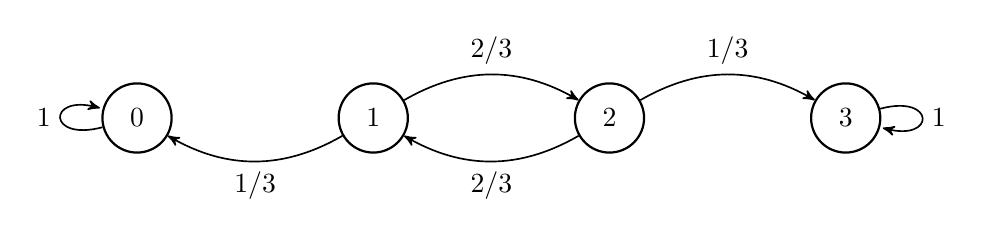
\begin{tikzpicture}[->, >=stealth', auto, semithick, node distance=3cm]
	\tikzstyle{every state}=[fill=white,draw=black,thick,text=black,scale=1]
	\node[state]    (A)                     {$0$};
	\node[state]    (B)[right of=A]   {$1$};
	\node[state]    (C)[right of=B]   {$2$};
	\node[state]    (D)[right of=C]   {$3$};
	\path
	(A) edge[loop left]			node{$1$}	(A)
	(B) edge[bend left,below]	node{$1/3$}	(A)
	edge[bend left,above]		node{$2/3$}	(C)
	(C) edge[bend left,below]	node{$2/3$}	(B)
	edge[bend left,above]		node{$1/3$}	(D)
	(D) edge[loop right]		node{$1$}	(D);
	%\node[above=0.5cm] (A){Patch G};
	%\draw[red] ($(D)+(-1.5,0)$) ellipse (2cm and 3.5cm)node[yshift=3cm]{Patch H};
	\end{tikzpicture}
\end{center}

\emph{Eine homogene, \textbf{irreduzible}, \textbf{aperiodische} Markov-Kette mit endlichem Zustandsraum ist immer \textbf{stationär}, d.h. sie konvergiert gegen ihr statistisches Gleichgewicht.}

\subsection{Übergangsmatrix}

\begin{itemize}
	\item Zeilen: Quelle, von diesem Knoten startet man
	\item Spalten: Zielknoten
	\item \(p_{ij}\) gibt dann die Übergangswahrscheinlichkeiten an
	\begin{itemize}
		\item \(p_{ij} \in [0;1] \rightarrow\) Es sind nur Werte zwischen 0 und 1 erlaubt
		\item \(\sum_{j=1}^{n} p_{ij} = 1 \rightarrow\) Die Summe der Zeilenwahrscheinlichkeiten \(=1\)
	\end{itemize}
\end{itemize}

\subsection{Stationäre Verteilung}
Ein Zustandsvektor \(\pi\) heißt \emph{stationäre Verteilung} einer Markov-Kette, wenn gilt:
\begin{equation*}
    \pi \cdot P = \pi
\end{equation*}

\(\lim_{n\rightarrow\infty} P^n\) konvergiert zur stationären Verteilung \(\pi\), wenn die Markov-Kette homogen, irreduzibel und aperiodisch ist.\\

Gleichungen lösen, ggf. mit Hilfe von Parametern \(t\), wenn es keine eindeutige Lösung gibt. Wert für \(t\) bestimmen, indem die Summe der Komponenten des Vektors \(\pi\) gleich 1 gesetzt wird.\\

\textbf{Beispiel:}
\begin{equation*}
    P = \begin{pmatrix}
        0.5 & 0.5\\
        0.3 & 0.7
    \end{pmatrix}
\end{equation*}
\begin{equation*}
    \begin{pmatrix}
        \pi_1 & \pi_2
    \end{pmatrix} \cdot \begin{pmatrix}
        0.5 & 0.5\\
        0.3 & 0.7
    \end{pmatrix} = \begin{pmatrix}
        \pi_1 & \pi_2
    \end{pmatrix}
\end{equation*}

Da \(\sum \pi_i=1\) gilt

\begin{equation*}
    \pi_1 + \pi_2 = 1 \Leftrightarrow \underline{\pi_1 = 1 - \pi_2} \Leftrightarrow \underline{\pi_2 = 1 - \pi_1}
\end{equation*}

\(\pi_1\) und \(\pi_2\) in die folgenden Gleichungen einsetzen:

\begin{equation*}
    \pi_1 \cdot 0.5 + \pi_2 \cdot 0.3 = \pi_1 \Longrightarrow \pi_2 = \frac{5}{8}
\end{equation*}
\begin{equation*}
    \pi_1 \cdot 0.5 + \pi_2 \cdot 0.7 = \pi_2 \Longrightarrow \pi_1 = \frac{3}{8}
\end{equation*}

Daraus folgt der stationäre Zustandsvektor: \(\pi = \begin{pmatrix}
    \frac{3}{8} & \frac{5}{8}
\end{pmatrix}\)



\subsection{Irreduzibilität}

Es ist von jedem Zustand aus möglich, jeden anderen Zustand zu erreichen.
Die Prüfung kann manuell erfolgen.\\

\textbf{Beispiel:}
\(
    P = \begin{pmatrix}
        1-p & p/2 & p/2\\
        1 & 0 & 0\\
        1 & 0 & 0
    \end{pmatrix}
\) ist irreduzibel für \(p\in (0,1]\), da für \(p=0\) Zustände 2 und 3 nicht mehr erreichbar sind.\\

Gegenteil = \emph{reduzibel}: Man kann die große Markovkette in kleinere Teile zerlegen (reduzieren), die nicht miteinander verbunden sind.\\

\subsection{Aperiodizität}

Die Periode eines Zustands ist die größte gemeinsame Teiler aller Pfade, die zu diesem Zustand zurück führen.\\

Starte in einem Zustand \(i\) und gehe in einen Zustand \(j\). Die Periode von \(i\) ist die größte gemeinsame Teiler aller Pfade, die von \(j\) nach \(i\) führen.
Wenn die Periode von jedem Zustand \(i\) gleich 1 ist, ist die Markov-Kette aperiodisch. Das heißt:

\begin{equation*}
    d(z)=ggT\{n \in \mathbb{N} | P_{ii}^{(n)} > 0\} = 1
\end{equation*}

\textbf{Beispiel:}
\(
    P = \begin{pmatrix}
        0 & 1\\
        1 & 0
    \end{pmatrix}
\) ist \emph{nicht} aperiodisch, da \(d(z) = 2\); man springt immer zwischen den beiden Zuständen mit einer geraden Anzahl hin und her.\\

\begin{center}
	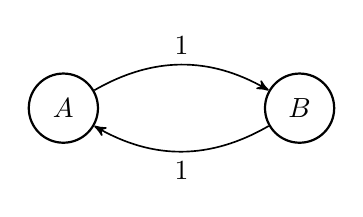
\begin{tikzpicture}[->, >=stealth', auto, semithick, node distance=3cm]
	\tikzstyle{every state}=[fill=white,draw=black,thick,text=black,scale=1]
	\node[state]    (A)               {$A$};
	\node[state]    (B)[right of=A]   {$B$};
	\path
	(A) edge[bend left]			node{$1$}	(B)
	(B) edge[bend left,below]	node{$1$}	(A);
	%\node[above=0.5cm] (A){Patch G};
	%\draw[red] ($(D)+(-1.5,0)$) ellipse (2cm and 3.5cm)node[yshift=3cm]{Patch H};
	\end{tikzpicture}
\end{center}

\textbf{Beispiel:}
\(
    P = \begin{pmatrix}
        1-p & p/2 & p/2\\
        1 & 0 & 0\\
        1 & 0 & 0
    \end{pmatrix}
\) ist aperiodisch für \(p\in [0,1)\), da bei \(p=1\) immer von Zustand 1 in 2 oder 3 gesprungen wird und wieder zurück.
Für alle anderen Werte wird in zwei Fällen auch hin- und zurückgesprungen. Allerdings gibt es auch die Möglichkeit, dass vom
Zustand \(A\) nicht geswechelt wird und man dort bleibt.\\

\begin{center}
	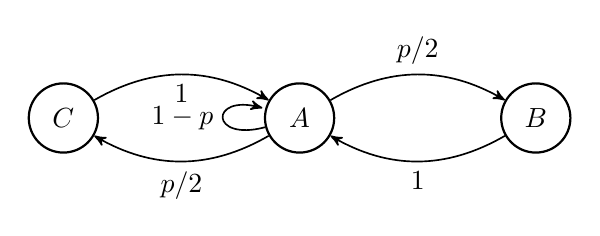
\begin{tikzpicture}[->, >=stealth', auto, semithick, node distance=3cm]
	\tikzstyle{every state}=[fill=white,draw=black,thick,text=black,scale=1]
	\node[state]    (A)               {$A$};
	\node[state]    (B)[right of=A]   {$B$};
	\node[state]    (C)[left of=A]    {$C$};
	% \node[state]    (D)[right of=C]   {$3$};
	\path
	(A) edge[loop left]			node{$1-p$}	(A)
    (A) edge[bend left]			node{$p/2$}	(B)
	(B) edge[bend left,below]	node{$1$}	(A)
    (A) edge[bend left, below]			node{$p/2$}	(C)
    (C) edge[bend left,below]	node{$1$}	(A);
	%\node[above=0.5cm] (A){Patch G};
	%\draw[red] ($(D)+(-1.5,0)$) ellipse (2cm and 3.5cm)node[yshift=3cm]{Patch H};
	\end{tikzpicture}
\end{center}

\subsection{Stoppzeiten}

Eine Stoppzeit ist eine Zufallsvariable, die das Eintreten eines Ereignisses beschreibt, das von der bisherigen Entwicklung eines stochastischen Prozesses abhängt.\\

\end{document}